\chapter{Introduction}

\section{Problem and motivation}

Every radiology image has to be described in words by a trained radiologist, and writing these descriptions takes time. \textbf{Image captioning} means generating such a description automatically: the model receives the pixels of an image and returns a sentence. An automatic first draft can save reporting effort and make descriptions more consistent.

The model works in two steps, like a radiologist who first studies the scan and then dictates one sentence: an \textbf{encoder} \emph{looks} at the image, and a \textbf{decoder} \emph{writes} the caption one word at a time (Figure 1.1).

\begin{figure}
\centering
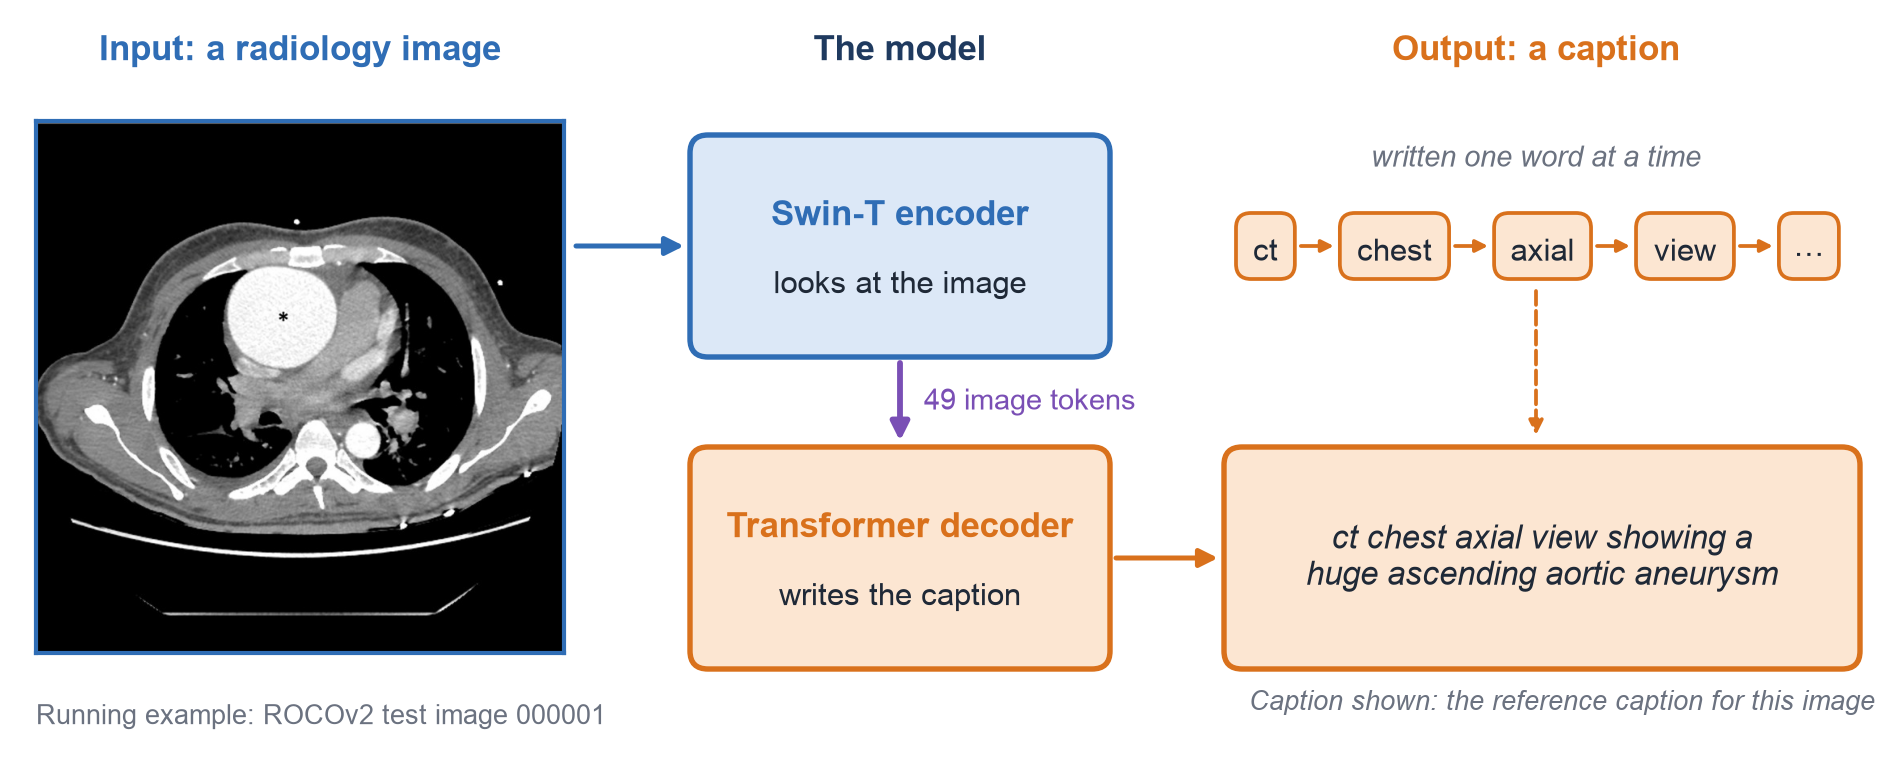
\includegraphics[width=1\linewidth,height=\textheight,keepaspectratio]{figures/fig1_1_task.png}
\caption{The captioning task. The Swin-T encoder turns the scan into 49 image tokens; the Transformer decoder uses them to write the caption one word at a time. This scan, ROCOv2 test image 000001, is the running example of the report.}
\end{figure}

Writing one word at a time follows from the chain rule of probability. The probability of a caption \(y = (y_1,\allowbreak \ldots,\allowbreak y_T)\) for an image \(I\) is the product of the probabilities of its words, each given the image and the words before it:

\[p(y | I) = \prod_{t=1}^{T} p\left(y_t | y_1, \ldots, y_{t-1}, I\right) \tag{1.1}\]

For example, if \(p(\text{ct} | I) = 0.6\) and \(p(\text{chest} | \text{ct},\allowbreak I) = 0.5\), then the caption ``ct chest'' (before the end token) has probability \(0.6 \times 0.5 = 0.3\).

\section{Challenges of medical captioning}

\begin{itemize}
\tightlist
\item
  \textbf{Small findings.} The important region is often a small part of the scan, so the model must keep track of \emph{where} things are.
\item
  \textbf{Specialised vocabulary.} Words such as \emph{pseudoaneurysm} or \emph{extravasation} are rare. Even after rare words are removed, the vocabulary has 8,729 tokens.
\item
  \textbf{Captions are figure legends.} ROCOv2 captions come from journal articles. They refer to arrows and panel letters, and some run to more than 100 words.
\item
  \textbf{Generic captions.} A model can score reasonably by always writing something safe, such as ``computed tomography scan of the chest showing a mass''. The share of \emph{distinct} captions has to be checked as well.
\end{itemize}

\needspace{33\baselineskip}

\section{Related work}

\begin{longtable}[]{@{}
  >{\raggedright\arraybackslash}p{(\linewidth - 4\tabcolsep) * \real{0.3333}}
  >{\raggedright\arraybackslash}p{(\linewidth - 4\tabcolsep) * \real{0.3333}}
  >{\raggedright\arraybackslash}p{(\linewidth - 4\tabcolsep) * \real{0.3333}}@{}}
\caption{Earlier work this project builds on.}\tabularnewline
\toprule\noalign{}
\begin{minipage}[b]{\linewidth}\raggedright
Work
\end{minipage} & \begin{minipage}[b]{\linewidth}\raggedright
Key idea
\end{minipage} & \begin{minipage}[b]{\linewidth}\raggedright
What we use from it
\end{minipage} \\
\midrule\noalign{}
\endfirsthead
\toprule\noalign{}
\begin{minipage}[b]{\linewidth}\raggedright
Work
\end{minipage} & \begin{minipage}[b]{\linewidth}\raggedright
Key idea
\end{minipage} & \begin{minipage}[b]{\linewidth}\raggedright
What we use from it
\end{minipage} \\
\midrule\noalign{}
\endhead
\bottomrule\noalign{}
\endlastfoot
Show and Tell {[}1{]} & CNN encodes the image as one vector; an LSTM writes the caption & Design of the CNN + LSTM baseline \\
Show, Attend and Tell {[}2{]} & The decoder looks at a grid of image regions for each word & The idea behind cross-attention \\
Transformer {[}3{]} & Attention instead of recurrence; masked self-attention, cross-attention & The decoder \\
ViT {[}4{]} & An image becomes a sequence of patches & Patch embedding \\
Swin Transformer {[}5{]} & Window attention, shifted windows, patch merging, pyramid & The encoder \\
ROCO {[}6{]}, ROCOv2 {[}7{]} & Radiology image--caption pairs from PubMed Central & The dataset \\
Lee et al.~{[}8{]} & Transformer captioning of medical images with global and local features & Closest related system \\
Pranay Kumar et al.~{[}9{]} & CNN + LSTM caption generator & Reference for the baseline \\
\end{longtable}

\section{Objectives}

\begin{enumerate}
\def\labelenumi{\arabic{enumi}.}
\tightlist
\item
  Build a radiology captioning model from a \textbf{Swin-T encoder} and a \textbf{6-layer Transformer decoder}.
\item
  Explain each component with intuition, equations, diagrams and small worked examples.
\item
  Train it on ROCOv2 with \textbf{transfer learning} and a \textbf{two-phase} schedule.
\item
  Evaluate it on the full test split (BLEU, ROUGE-L, CIDEr-D, METEOR, distinct captions) and compare it with a \textbf{CNN + LSTM baseline}.
\end{enumerate}

\textbf{How to read this report.} Chapter 2 prepares the data. Chapter 3 follows one image and one caption through the model, step by step. Chapters 4--9 cover the baseline, metrics, results and conclusions. In every figure, blue marks the image and encoder, orange the words and decoder, purple attention, green MLP layers, and red masked positions. Figures marked \emph{illustration} use made-up numbers to explain an idea.
